% !TeX spellcheck = pl_PL

\newpage
%===============================================================================
%*** Opracowanie wykładów *****************************
%===============================================================================
\part{Teoria}


%========================================
%*** Historia rozwoju komputerów ********
%========================================
\section{Historia rozwoju komputerów}
	\begin{enumerate}
	    \item Liczydło
	    \item Pascalina - maszyna licząca Pascala (dodawanie i odejmowanie)
	    \item Maszyna mnożąca Leibniza (dodawanie, odejmowanie, mnożenie, dzielenie, pierwiastek kwadratowy
	    \item Maszyna różnicowa - Charles Babbage, obliczanie wartości matematycznych do tablic
	    \item Maszyna analityczna - Charles Babvage, programowalna za pomocą kart perforowanych
	  	\item Elektryczna maszyna sortująca i tabelaryzująca Holleritha 1890
	    \item Kalkulator elektromechaniczny Mark I, tablicowanie funkcji, całkowanie numeryczne, rozwiązywanie równań różniczkowych, rozwiązywanie układów równań liniowych, analiza harmoniczna, obliczenia statystyczne
	    \item Maszyny liczące Z1: pamięć mechaniczna, zmiennoprzecinkowa reprezentacja liczb, binarna jednostka zmiennoprzecinkowa
	    \item Z3: Pierwsza maszyna w pełni automatyczna, kompletna w sensie Turinga, pamięć przekaźnikowa
	    \item Colossus i Colossus 2
	    \item ENIAC
	    \item EDVAC - J. von Neumann (wtedy utworzył swoją architekturę) \\
	    	\begin{figure}[h]
			\centering
			%\includegraphics[scale=0.1]{architektura_von_Neumanna.png}
			\end{figure}
	    \item UNIVAC I (pierwszy udany komputer komercyjny)
	    \item IBM 701, potem 709
	    \item po 1955 zaczyna się zastosowanie tranzystorów w komputerach (komputery II generacji)
	    \item po 1965 komputery III generacji z układami scalonymi
	    \item od 1971 komputery IV generacji - z układami scalonymi wielkiej skali inegracji VLSI
    \end{enumerate}
    

%========================================
%*** Architektura CISC ******************
%========================================
\section{Architektura CISC}
	\subsection{Znaczenie} \noindent
		Complex Instruction Set Computers
	
	\subsection{Przyczyny rozwoju architektury CISC}
    	\begin{itemize}
	        \item Drogie, małe i wolne pamięci komputerów
	        \item Rozwój wielu rodzin komputerów
	        \item Duża popularność mikroprogramowalnych układów sterujących (prostych w rozbudowie)
	        \item Dążenie do uproszczenia kompilatorów. Im więcej będzie rozkazów maszynowych odpowiadających instrukcjom języków wyższego poziomu tym lepiej.
        \end{itemize}
    
    \subsection{Cechy architektury CISC}
    	\begin{itemize}
	        \item Duża liczba rozkazów (z czego te najbardziej zaawansowane i tak nie były używane)
	        \item Duża ilość trybów adresowania (związane z modelem obliczeń)
	        \item Duży rozrzut cech rozkazów w zakresie:
	        \begin{itemize}
		        \item złożoności
		        \item długości (szczególnie to - nawet kilkanaście bajtów)
		        \item czasów wykonania
	        \end{itemize}
	        \item Model obliczeń pamięć - pamięć
	        \item Niewiele rejestrów - były droższe niż komórki pamięci i przy przełączaniu kontekstu obawiano się wzrostu czasu przełączania kontekstu (chowanie rejestrów na stos i odwrotnie)
        \end{itemize}
   
   \textbf{\large CIEKAWOSTKA:} Przeanalizowano jakieś tam programy i w procesorze VAX 20\% najbardziej złożonych rozkazów odpowiadało za 60\% kodu, stanowiąc przy tym ok 0.2\% wywołań.\\ W procesorze MC68020 71\% rozkazów nie zostało nawet użytych w badanych programach
   
	\section{Architektura RISC}
		\subsection{Znaczenie} \noindent
			Reduced Instruction Set Computers
   		\subsection*{Przyczyny rozwoju}
	   		\begin{itemize}
	   			\item Poszukiwanie optymalnej listy rozkazów
	   			\item Chęć wykonania mikroprocesora o funkcjach pełnego ówczesnego procesora
	   		\end{itemize}
   		
   		\subsection{Pierwszy procesor RISC} \noindent
	   		Procesor RISC I (1980), D. Patterson (Berkeley University)\\
	   		Założenia projektowe:
	   		\begin{itemize}
	   			\item Wykonanie jednego rozkazu w jednym cyklu maszynowym
	   			\item Stały rozmiar rozkazów – uproszczenie metod adresacji
	   			\item Model obliczeń rejestr – rejestr: komunikacja z pamięcią operacyjną tylko za pomocą rozkazów LOAD i STORE.
	   			\item Wsparcie poprzez architekturę języków wysokiego poziomu.
	   		\end{itemize}
	   		Efekty realizacji fizycznej:
	   		\begin{itemize}
	   			\item 44 420 tranzystorów (ówczesne procesory CISC zawierały ok. 100 000 tranzystorów)
	   			\item lista rozkazów = 32 rozkazy
	   			\item dwustopniowy potok – strata tylko 6\% cykli zegara, zamiast 20\% (w związku z realizacją skoków)
	   		\end{itemize}
   		
   		\subsection{Cechy architektury RISC}
	   		\begin{enumerate}
	   			\item Stała długość i prosty rozkaz formatu
	   			\item Nieduża liczba trybów adresowania
	   			\item Niezbyt obszerna lista rozkazów
	   			\item Model obliczeń rejestr-rejestr - dostęp do pamięci operacyjnej tylko w rozkazach LOAD i STORE
	   			\item Duży zbiór rejestrów uniwersalnych
	   			\item Układ sterowania – logika szyta
	   			\item Intensywne wykorzystanie przetwarzania potokowego
	   			\item Kompilatory o dużych możliwościach optymalizacji potoku rozkazów
	   		\end{enumerate}
   		
   		\subsection{Format rozkazu procesora RISC I}
	   		\begin{table}[h]
	   			\begin{tabular}{clclll}
	   				\hline
	   				\multicolumn{1}{|c|}{7}      & \multicolumn{1}{c|}{1}   & \multicolumn{1}{c|}{5}    & \multicolumn{1}{c|}{5}    & \multicolumn{1}{c|}{1}   & \multicolumn{1}{c|}{13}   \\ \hline
	   				\multicolumn{1}{|c|}{OPCODE} & \multicolumn{1}{c|}{SCC} & \multicolumn{1}{c|}{DEST} & \multicolumn{1}{c|}{SRC1} & \multicolumn{1}{c|}{IMM} & \multicolumn{1}{c|}{SRC2} \\ \hline
	   			\end{tabular}
	   		\end{table}
	   		\begin{itemize}
	   			\item OPCODE–kod rozkazu
	   			\item SCC – ustawianie (lub nie) kodów warunków
	   			\item DEST – nr rejestru wynikowego
	   			\item SRC1 – nr rejestru zawierającego pierwszy argument
	   			\item IMM – wskaźnik natychmiastowego trybu adresowania
	   			\item SRC2 – drugi argument lub nr rejestru (na 5 bitach)
	   		\end{itemize}
   		
   		\subsection{Realizacja wybranych rozkazów}
   			\subsubsection{Rozkazy arytmetyczne}
	   			\begin{itemize}
	   				\item \textbf{Tryb rejestrowy}:\tab(IMM=0) \tab R[DEST] $\leftarrow$ R[SRC1] op R[SRC2]
	   				\item \textbf{Tryb natychmiastowy:}\tab(IMM=1) \tab{R[DEST] $\leftarrow$ R[SRC1] op SRC2}
	  			\end{itemize}
        	\subsubsection{Rozkazy komunikujące się z pamięcią}
	        	\begin{itemize}
	        		\item \textbf{LOAD}\tab{R[DEST] $\leftarrow$ M[AE]P}
	        		\item \textbf{STORE}\tab{M[AE]  $\leftarrow$ R[DEST]}
	        	\end{itemize}
        	\subsubsection{Adres efektywny}
	        	\begin{itemize}
	        		\item \textbf{Tryb z przesunięciem}\tab\tab AE = R[SRC1] + SRC2 = RX + S2
	        		\item \textbf{Inny zapis powyższego}\tab\tab AE = RX + S2
	        		\item \textbf{Tryb absolutny}\tab\tab AE = R0 + S2 = S2 (R0 $\equiv$ 0)
	        		\item \textbf{Tryb rejestrowy pośredni}\tab AE = RX + 0 = RX
	        	\end{itemize}
	        	Tryb absolutny oraz tryb rejestrowy pośredni są przypadkami szczególnymi.

	\newpage
    \subsection{Logiczna organizacja rejestrów procesora RISC I}
	    \begin{table}[htbp]
	    	\centering
	    	\caption{Rejestry}
	    	\begin{tabular}{c|c|c}
	    		\cline{2-2}    \multirow{4}[2]{*}{6} & \multirow{4}[2]{*}{Wysokie} & {\scriptsize R31} \bigstrut[t]\\
	    		&       &  \\
	    		&       &  \\
	    		&       &  \bigstrut[b]\\
	    		\cline{2-2}    \multirow{4}[2]{*}{10} & \multirow{4}[2]{*}{Lokalne} &  \bigstrut[t]\\
	    		&       &  \\
	    		&       &  \\
	    		&       &  \bigstrut[b]\\
	    		\cline{2-2}    \multirow{4}[2]{*}{6} & \multirow{4}[2]{*}{Niskie} &  \bigstrut[t]\\
	    		&       &  \\
	    		&       &  \\
	    		&       &  \bigstrut[b]\\
	    		\cline{2-2}    \multirow{4}[2]{*}{10} & \multirow{4}[2]{*}{Globalne} & {\scriptsize R9} \bigstrut[t]\\
	    		&       &  \\
	    		&       &  \\
	    		&       & {\scriptsize R0} \bigstrut[b]\\
	    		\cline{2-2}    \end{tabular}%
	    	\label{tab:addlabel}%
	    	\vspace{-2cm}
	    \end{table}
	\subsection{Okno rejestrów}
	    \begin{table}[htbp]
	    	\centering
	    	\caption{Rejestry fizyczne}
	    	\begin{tabular}{r|r|r}
	    		\cline{2-2}    137   & \multirow{6}[2]{*}{$ \uparrow $ Okno rejestrów} &  \bigstrut[t]\\
	    		&       &  \\
	    		&       &  \\
	    		&       &  \bigstrut[b]\\
	    		\cline{2-2}          & \multicolumn{1}{c|}{\multirow{4}[2]{*}{Wysokie}} & \multicolumn{1}{c}{R31} \bigstrut[t]\\
	    		& \multicolumn{1}{c|}{} & \multicolumn{1}{c}{} \\
	    		& \multicolumn{1}{c|}{} & \multicolumn{1}{c}{} \\
	    		& \multicolumn{1}{c|}{} & \multicolumn{1}{c}{} \bigstrut[b]\\
	    		\cline{2-2}          & \multicolumn{1}{c|}{\multirow{4}[2]{*}{Lokalne}} & \multicolumn{1}{c}{} \bigstrut[t]\\
	    		& \multicolumn{1}{c|}{} & \multicolumn{1}{c}{} \\
	    		& \multicolumn{1}{c|}{} & \multicolumn{1}{c}{} \\
	    		& \multicolumn{1}{c|}{} & \multicolumn{1}{c}{} \bigstrut[b]\\
	    		\cline{2-2}          & \multicolumn{1}{c|}{\multirow{4}[2]{*}{Niskie}} & \multicolumn{1}{c}{} \bigstrut[t]\\
	    		& \multicolumn{1}{c|}{} & \multicolumn{1}{c}{} \\
	    		& \multicolumn{1}{c|}{} & \multicolumn{1}{c}{} \\
	    		& \multicolumn{1}{c|}{} & \multicolumn{1}{c}{} \bigstrut[b]\\
	    		\cline{2-2}          & \multicolumn{1}{c|}{\multirow{4}[2]{*}{Globalne}} & \multicolumn{1}{c}{} \bigstrut[t]\\
	    		& \multicolumn{1}{c|}{} & \multicolumn{1}{c}{} \\
	    		& \multicolumn{1}{c|}{} & \multicolumn{1}{c}{} \\
	    		& \multicolumn{1}{c|}{} & \multicolumn{1}{c}{R0} \bigstrut[b]\\
	    		\cline{2-2}          & \multicolumn{1}{c|}{\multirow{2}[2]{*}{$ \downarrow $ }} &  \bigstrut[t]\\
	    		& \multicolumn{1}{c|}{} &  \\
	    		0     & \multicolumn{1}{c|}{} &  \bigstrut[b]\\
	    		\cline{2-2}
	    	\end{tabular}%
	    	\label{tab:addlabel}%
	    \end{table}
	    
	    % --- OBRAZKI
%	    \begin{center}
%	    	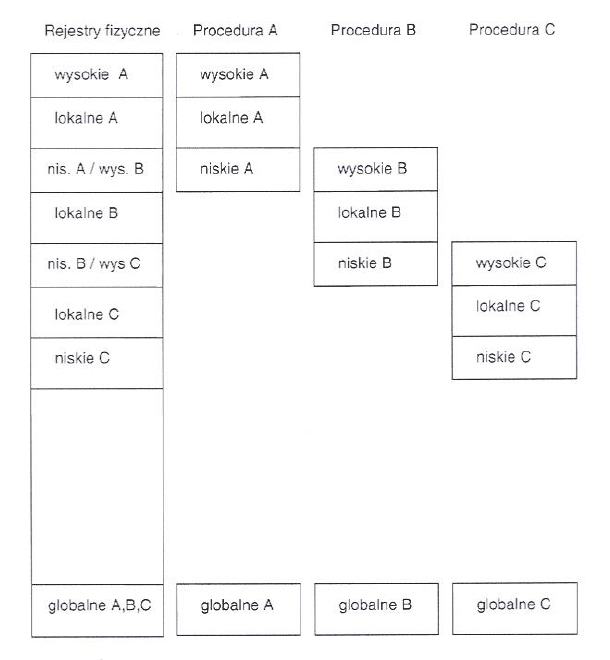
\includegraphics[width=10cm]{RISC_proc1}
%	    \end{center}
%	    \begin{center}
%	    	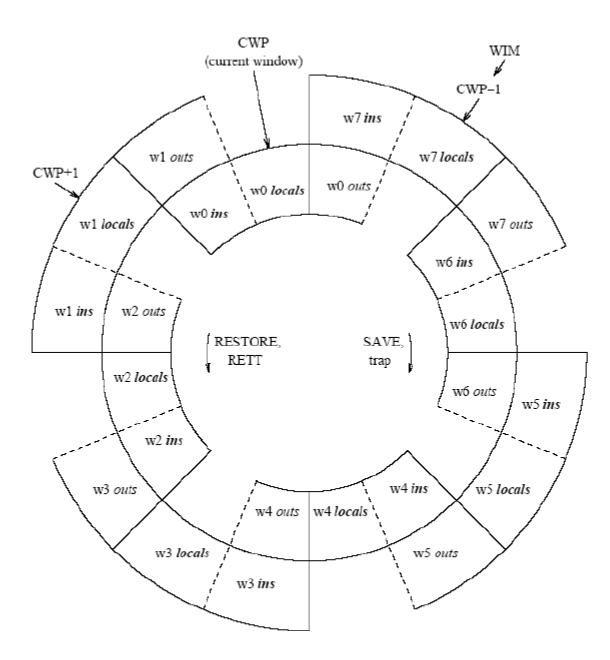
\includegraphics[width=10cm]{RISC_proc2}
%	    \end{center}
	    
	\pagebreak
\section{Mechanizmy potokowe}
	\subsection{Realizacja rozkazów w procesorze niepotokowym}
		Rozkazy wykonywane są liniowo w czasie - jeden po drugim, w takiej kolejności w jakiej przyjdą do procesora.
   	\subsection{Potokowe wykonanie rozkazówdla prostej organizacji cyklu rozkazowego}
   		Prosty podział procesora na moduły:
	   	\begin{itemize}
	   		\item S1 - pobranie rozkazu
	   		\item S2 - wykonanie rozkazu
	   	\end{itemize}
   		Zakładając, że czas pracy obu modułów jest równy, wówczas 3 rozkazy mogą zostać wykonane w 2 okresach.\\
   		1 T - pobranie i wykonanie rozkazu. W momencie gdy pierwszy rozkaz zostanie pobrany, w chwili 0.5 T S1 może pobrać kolejny.
   	\subsection{Podział cyklu rozkazowego na większą liczbę faz}
   		Na przykładzie cyklu rozkazowego komputera Amdahl 470
	   	\begin{enumerate}
	   		\item Pobranie rozkazu
	   		\item Dekodowanie rozkazu
	   		\item Obliczenie adresu efektywnego
	   		\item Pobranie argumentów
	   		\item Wykonanie operacji
	   		\item Zapis wyniku
	   	\end{enumerate}
	   	Zasada działania jest dokładnie taka sama jak w przypadku podziału na dwie fazy. Załóżmy, że jeden rozkaz wykonuje się w 7iu taktach zegarowych. 1 T = 7 F. Wówczas w momencie gdy rozkaz numer 1 znajduje się w 5tym takcie wykonania rozkaz numer 5 może zostać pobrany.
   
	   	\begin{table}[htbp]
	   		\centering
	   		\caption{Zobrazowanie potoku}
	   		\begin{tabular}{|r|r|r|r|r|r|r|r|r|}
	   			\multicolumn{1}{r}{Rozkazy} & \multicolumn{1}{r}{} & \multicolumn{7}{c}{Fazy zegarowe} \\
	   			\multicolumn{1}{r}{} & \multicolumn{1}{r}{} & \multicolumn{1}{c}{1} & \multicolumn{1}{c}{2} & \multicolumn{1}{c}{3} & \multicolumn{1}{c}{4} & \multicolumn{1}{c}{5} & \multicolumn{1}{c}{6} & \multicolumn{1}{c}{7} \bigstrut[b]\\
	   			\cline{1-1}\cline{3-9}    \multicolumn{1}{|c|}{S1} &       & r1    & r2    & r3    & r4    & r5    & r6    & r7 \bigstrut\\
	   			\cline{1-1}\cline{3-9}    \multicolumn{1}{|c|}{S2} &       &       & r1    & r2    & r3    & r4    & r5    & r6 \bigstrut\\
	   			\cline{1-1}\cline{3-9}    \multicolumn{1}{|c|}{S3} &       &       &       & r1    & r2    & r3    & r4    & r5 \bigstrut\\
	   			\cline{1-1}\cline{3-9}    \multicolumn{1}{|c|}{S4} &       &       &       &       & r1    & r2    & r3    & r4 \bigstrut\\
	   			\cline{1-1}\cline{3-9}    \multicolumn{1}{|c|}{S5} &       &       &       &       &       & r1    & r2    & r3 \bigstrut\\
	   			\cline{1-1}\cline{3-9}    \multicolumn{1}{|c|}{S6} &       &       &       &       &       &       & r1    & r2 \bigstrut\\
	   			\cline{1-1}\cline{3-9}    \end{tabular}%
	   		\label{tab:addlabel}%
	   	\end{table}%
	   
   	\subsection{Analiza czasowa potokowej realizacji ciągu rozkazów}
   		Założenia
	   	\begin{itemize}
	   		\item \textbf{P} - liczba faz
	   		\item \textbf{T} - okres
	   		\item $\frac{T}{P}=\tau $ - czas wykonania pojedynczej fazy
	   	\end{itemize}
   		$(n-1)\times\tau$ - czas rozpoczęcia wykonywania \emph{n}-tego rozkazu.
   	\subsection{Czas wykonywania rozkazów}
	   	\begin{itemize}
	   		\item W procesorze niepotokowym\\
	   		$t=n\times T$ - dla \emph{n} rozkazów
	   		\item W procesorze potokowym dla idealnego przypadku, gdy $\tau=\frac{T}{P}$\\
	   		$t=(n-1)\times\tau+T=(n-1+P)\times\frac{T}{P}$
	   	\end{itemize}
   	\subsection{Przyspieszenie dla potokowego wykonania rozkazów}
	   	Przyspieszenie jest stosunkiem czasu wykonywania rozkazów dla procesora niepotokowego do czasu dla procesora potokowego.\\\\
	   	$\lim_{n \to \infty}\frac{n\times T}{(n-1+P)\times\frac{T}{P}}=P$\\\\
	   	Maksymalne przyspieszenie (dla modelu idealnego) jest równe ilości faz.
   	\subsection{Problemy z potokową realizacją rozkazów}
   		Problemem związanym z realizacją potokową jest \textbf{zjawisko hazardu}.
	   	\begin{itemize}
	   		\item \textbf{Hazard sterowania }– problemy z potokową realizacją skoków i rozgałęzień.
	   		\item \textbf{Hazard danych} – zależności między argumentami kolejnych rozkazów
	   		\item \textbf{Hazard zasobów} – konflikt w dostępie do rejestrów lub do pamięci
	   	\end{itemize}
   	\subsection{Rozwiązanie problemu hazardu sterowania}
	   	\begin{itemize}
	   		\item Skoki opóźnione
	   		\item Przewidywanie rozgałęzień
	   	\end{itemize}
   	\subsection{Skoki opóźnione}
	   	\subsubsection{Założenia}
		   	\begin{itemize}
		   		\item Rozkaz następny po skoku jest zawsze całkowicie wykonywany
		   		\item To znaczy, że efekt skoku jest opóźniony o jeden rozkaz
		   	\end{itemize}
   		\subsubsection{Działanie}
   			Zmienia kod programu w trakcie kompilacji, jeśli widzi taka potrzebę. Sprowadza się to do dwóch możliwości:
		   	\begin{itemize}
		   		\item Modyfikacja programu - dodanie rozkazu NOP po instrukcji skoku JMP
		   		\item Optymalizacja programu - zmiany kolejności wykonywania rozkazów
		   	\end{itemize}
   	\subsection{Przewidywanie rozgałęzień}
	   	\begin{enumerate}
	   		\item Strategie statyczne
	   		\begin{itemize}
	   			\item przewidywanie, że rozgałęzienie (skok warunkowy) zawsze nastąpi
	   			\item przewidywanie, że rozgałęzienie nigdy nie nastąpi
	   			\item podejmowanie decyzji na podstawie kodu rozkazu rozgałęzienia (specjalny bit ustawiany przez kompilator)
	   		\end{itemize}
	   		\item Inne strategie
	   		\begin{itemize}
	   			\item przewidywanie, że skok wstecz względem licznika rozkazów zawsze nastąpi
	   			\item przewidywanie, że skok do przodu względem licznika rozkazów nigdy nie nastąpi
	   		\end{itemize}
	   		\item Strategie dynamiczne
	   		\begin{itemize}
	   			\item Tablica historii rozgałęzień.
	   		\end{itemize}
	   		\subsubsection{Tablica historii rozgałęzień}
	   		Składa się z:
	   		\begin{itemize}
	   			\item Bit ważności
	   			\item Adres rozkazu rozgałęzienia
	   			\item Bity historii
	   			\item Adres docelowy rozgałęzienia (opcja)
	   		\end{itemize}
	   		Operacje wykonywane na tablicy historii rozgałęzień
	   		\begin{itemize}
	   			\item Sprawdzenie, czy adres rozkazu rozgałęzienia jest w tablicy
	   			\begin{itemize}
	   				\item \textbf{Nie} – wtedy:
	   				\begin{itemize}
	   					\item przewidywanie rozgałęzienia jest wykonywane według jednej ze strategii statycznych
	   					\item do tablicy jest wpisywany adres rozkazu rozgałęzienia, informacja o wykonaniu/niewykonaniu rozgałęzienia (bit historii) i (opcjonalnie) adres docelowy rozgałęzienia
	   				\end{itemize}
	   				\item \textbf{Tak} - wtedy:
	   				\begin{itemize}
	   					\item przewidywanie rozgałęzienia jest wykonywane według bitów historii
	   					\item do tablicy jest wpisywana informacja o wykonaniu/niewykonaniu rozgałęzienia (uaktualnienie bitów historii)
	   				\end{itemize}
	   			\end{itemize}
	   			\item 1 bit historii - algorytm przewidywania rozgałęzień dla jednego bitu historii - kolejne wykonanie rozkazu rozgałęzienia będzie przebiegało tak samo jak poprzednie.
	   			\item 2 bity historii
	   			\begin{itemize}
	   				\item algorytm przewidywania rozgałęzień dla dwóch bitów historii bazuje na 2-bitowym automacie skończonym.
	   				\item Interpretacja dwóch bitów historii (x y):
	   				\begin{itemize}
	   					\item y: historia ostatniego wykonania skoku (0 – nie, 1 – tak)
	   					\item x: przewidywanie następnego wykonania skoku (0 – nie, 1 – tak)
	   					\item Ogólna zasada przewidywania - zmiana strategii następuje dopiero po drugim błędzie przewidywania.
	   				\end{itemize}
	   			\end{itemize}
	   		\end{itemize}
	   	\end{enumerate}

	\subsection{Metody rozwiązywania hazardu danych}
		\subsubsection{Co to jest?}
			Hazard danych - zależności między argumentami kolejnych rozkazów wykonywanych potokowo.
		\subsubsection{Metody usuwania hazardu danych}
			Jest kilka sposobów:
			\begin{itemize}
			   		\item Sprzętowe wykrywanie zależności i wstrzymanie napełniania potoku
			   		\item Wykrywanie zależności na etapie kompilacji i modyfikacja programu (np. dodanie rozkazu NOP)
			   		\item Wykrywanie zależności na etapie kompilacji, modyfikacja i optymalizacja programu (np. zamiana kolejności wykonywania rozkazów)
			   		\item Wyprzedzające pobieranie argumentów (zastosowanie szyny zwrotnej)
			\end{itemize}
		\subsubsection{Problem}
			Jeśli faza wykonania rozkazu nie będzie mogła być wykonana w jednym takcie (np. dla rozkazów zmiennoprzecinkowych), to zachodzi konieczność wstrzymania napełniania potoku.
        	

\section{Architektura superskalarna}
	\subsection{Co to jest?}
		Architektura umożliwiająca wykonanie w jednym takcie większej od 1 liczby instrukcji.
	   	\subsection*{Cechy architektury superskalarnej}
	       	\begin{itemize}
	        	\item Możliwość wykonania kilku rozkazów w jednym takcie, co powoduje konieczność:
			    \begin{itemize}
		          	\item Kilku jednostek potokowych
		         	\item Załadowania kilku rozkazów z pamięci operacyjnej w jednym takcie procesora
			    \end{itemize}
	        \end{itemize}
	
    \subsection{Zależności między rozkazami}
       	\begin{itemize}
         \item \textbf{Prawdziwa zależność danych} - \emph{Read After Write (RAW)}\\
         Występuje w momencie kiedy jeden rozkaz wymaga argumentu obliczanego przez poprzedni rozkaz. Opóźnienie eliminowane za pomocą "wyprzedzającego pobierania argumentu" - dana nie jest zapisywana do rejestru, tylko pobierana bezpośrednio z poprzedniego rozkazu, który znajduje się w akumulatorze (jeżeli dobrze rozumiem rysunek ze slajdu 21, wykład 4)
         \item \textbf{Zależność wyjściowa} - \emph{Write After Write (WAW)}\\
         Gdy rozkazy zapisująca dane do tego samego rejestru wykonują się równolegle to drugi z nich musi czekać aż pierwszy się zakończy. Układ sterujący musi kontrolować tego typu zależność.
         \item \textbf{Antyzależność} - \emph{Write After Read (WAR)}\\
         W przypadku gdy pierwszy rozkaz czyta wartość rejestru, a drugi zapisuje coś do tego rejestru i oba wykonują się równolegle, to drugi musi czekać aż pierwszy odczyta swoje.
        \end{itemize}
        \subsubsection*{Wnioski}
	        \begin{itemize}
	           	\item Dopuszczenie do zmiany kolejności rozpoczynania wykonania (wydawania) rozkazów i / lub zmiany kolejności kończenia rozkazów prowadzi do możliwości wystąpienia zależności wyjściowej lub antyzależności.
	           	\item Zawartości rejestrów nie odpowiadają wtedy sekwencji wartości, która winna wynikać z realizacji programu
	        \end{itemize}
        
	\subsection{Metody eliminacji zależności}
		\begin{enumerate}
			\item Metoda przemianowania rejestrów
			\begin{itemize}
				\item Stosowana w przypadku zwielokrotnienia zestawu rejestrów.
				\item Rejestry są przypisywane dynamicznie przez procesor do rozkazów.
				\item Gdy wynik rozkazu ma być zapisany do rejestru Rn, procesor angażuje do tego nową kopię tego rejestru.
				\item Gdy kolejny rozkaz odwołuje się do takiego wyniku (jako argumentu źródłowego), rozkaz ten musi przejść przez proces przemianowania.
				\item Przemianowanie rejestrów eliminuje antyzależność i zależność wyjściową.
			\end{itemize}
		\end{enumerate}
		
\section{Architektura VLIW}
	\subsection{Co to jest?}
		VLIW - Very Long Instruction Word.
	\subsection{Cechy}
		\begin{itemize}
			\item Wspólna pamięć operacyjna
			\item Szeregowanie rozkazów
		\end{itemize}
	\subsection{Szeregowanie rozkazów przez kompilator}
		\begin{itemize}
			\item Podział rozkazów programu na grupy
			\item Sekwencyjne wykonywanie grup
			\item Możliwość równoległej realizacji rozkazów w ramach grupy
			\item Podział grupy na paczki
			\item Paczka = 3 rozkazy + szablon (3 x 41 + 5 = 128 bitów)
			\item Szablon - informacja o jednostkach funkcjonalnych, do których kierowane mają być rozkazy i ewentualna informacja o granicach grup w ramach paczki
		\end{itemize}
	\subsection{Redukcja skoków warunkowych - predykacja rozkazów}
		Rozkazy uwarunkowane - uwzględnianie warunku w trakcie realizacji rozkazu.
	\subsection{Spekulatywne wykonanie rozkazów LOAD}
		\begin{itemize}
			\item Problem: chybione odwołania do PaP (cache) i konieczność czekania na sprowadzenie do PaP linii danych
			\item Rozwiązanie: przesunięcie rozkazów LOAD jak najwyżej, aby zminimalizować czas ewentualnego oczekiwania.
			\item Rozkaz CHECK sprawdza wykonanie LOAD (załadowanie rejestru)
		\end{itemize}
	
\section{Wielowątkowość}
	\subsection{Co to jest?}
		\begin{itemize}
			\item Cecha systemu operacyjnego umożliwiająca wykonywanie kilku wątków w ramach jednego procesu
			\item Cecha procesora oznaczająca możliwość jednoczesnego wykonywanie kilku wątków w ramach jednego procesora (rdzenia)
		\end{itemize}
	\subsection{Sprzętowa realizacja wielowątkowości}
		Celem współbieżnej realizacji dwóch (lub więcej) wątków w jednym procesorze (rdzeniu) jest minimalizacja strat cykli powstałych w trakcie realizacji pojedynczego wątku w wyniku:
		\begin{itemize}
			\item chybionych odwołań do pamięci podręcznej,
			\item błędów w przewidywaniu rozgałęzień,
			\item zależności między argumentami kolejnych rozkazów
		\end{itemize}
	\subsection{Wielowątkowość gruboziarnista}
		Coarse-grained multithreading
		\begin{itemize}
			\item Przełączanie wątków następuje przy dłuższym opóźnieniu wątku w potoku (np. chybione odwołanie do pamięci podręcznej (nawet L2))
			\item W niektórych rozwiązaniach rozpoczęcie nowego wątku następuje dopiero po opróżnieniu potoku
			\item Zaletą jest prostota procesu przełączania wątków
			\item Wadą takiego rozwiązania są straty czasu przy krótszych opóźnieniach potoku
		\end{itemize}
	\subsection{Wielowątkowość drobnoziarnista}
		Fine-grained multithreading
		\begin{itemize}
			\item Przełączanie wątków następuje po każdym rozkazie
			\item Wątek oczekujący (np. na dostęp do pamięci) jest pomijany
			\item Zaletą jest unikanie strat nawet przy krótkich opóźnieniach wątków
			\item Istotnym wymaganiem dla procesora jest szybkie (w każdym takcie) przełączanie wątków
			\item Pewną wadą jest opóźnienie realizacji wątków w pełni gotowych do wykonania
		\end{itemize}
	\subsection{Warunki sprzętowej realizacji wielowątkowości}
		\begin{itemize}
			\item powielenie zestawów rejestrów uniwersalnych (lub powielenie tabel mapowania rejestrów)
			\item powielenie liczników rozkazów
			\item powielenie układów dostępu do pamięci podręcznej (tabel stron)
			\item powielenie sterowników przerwań
		\end{itemize}
	\subsection{Wielowątkowość w procesorze dwupotokowym}
		Reguły realizacji i przełączania wątków:
		\begin{enumerate}
			\item Wielowątkowość gruboziarnista
			\begin{itemize}
				\item wątek realizowany w kolejnych taktach do momentu wstrzymania rozkazu
				\item do obu potoków wprowadzane są rozkazy tylko jednego wątku (w jednym takcie!)
			\end{itemize}
			\item Wielowątkowość drobnoziarnista
			\begin{itemize}
				\item w kolejnych taktach realizowane są naprzemiennie rozkazy kolejnych wątków (przełączanie wątków co takt)
				\item do obu potoków wprowadzane są rozkazy tylko jednego wątku (w jednym takcie!)
			\end{itemize}
			\item Wielowątkowość współbieżna (SMT -Simultaneous multithreading)
			\begin{itemize}
				\item wątek realizowany do momentu wstrzymania rozkazu
				\item do obu potoków w jednym takcie mogą być wprowadzane rozkazy różnych wątków
			\end{itemize}
		\end{enumerate}
	\subsection{Mankamenty współbieżnej wielowątkowości}
		\begin{itemize}
			\item Rywalizacja wątków w dostępie do pamięci podręcznej - mniejsza wielkość PaP przypadająca na wątek
			\item Większe zużycie energii (w porównaniu z procesorami dwurdzeniowymi)
			\item Możliwość monitorowanie wykonania jednego wątku przez inny wątek (złośliwy), poprzez wpływ na współdzielone dane pamięci podręcznej - kradzież kluczy kryptograficznych
		\end{itemize}

\section{Klasyfikacja komputerów równoległych}
	\subsection{Formy równoległości w architekturze komputerów}
		\subsubsection{Równoległość na poziomie rozkazów}
			Wykonywanie w danej chwili wielu rozkazów w jednym procesorze.
			\begin{itemize}
				\item Mechanizmy potokowe - w procesorach CISC i RISC
				\item Architektura superskalarna i VLIW
			\end{itemize}
		\subsubsection{Równoległość na poziomie procesorów}
			Wykonywanie w danej chwili wielu rozkazów w wielu procesorach.
			\begin{itemize}
				\item Komputery wektorowe
				\item Komputery macierzowe
				\item Systemy wieloprocesorowe
				\item Klastry (systemy wielokomputerowe)
			\end{itemize}
	\subsection{Rodzaje równoległości w aplikacjach}
		\subsubsection{Równoległość poziomu danych}
			DLP - Data Level Parallelism.\\
			Pojawia się kiedy istnieje wiele danych, które mogą być przetwarzane w tym samym czasie.
		\subsubsection{Rówoległość poziomu zadań}
			TLP - Task Level Parallelism.\\
			Pojawia się kiedy są tworzone zadania, które mogą być wykonywane niezależnie i w większości równolegle.
	
	\subsection{Drogi wykorzystania równoległości aplikacji w architekturze komputerów}
		\begin{itemize}
			\item \textbf{Równoległość poziomu rozkazów} (ILP - Instruction Level Parallelism) - odnosi się do przetwarzania potokowego i superskalarnego, w których w pewnym (niewielkim) stopniu wykorzystuje się równoległość danych.
			\item \textbf{Architektury wektorowe i procesory graficzne} - wykorzystują równoległość danych poprzez równoległe wykonanie pojedynczego rozkazu na zestawie danych.
			\item \textbf{Równoległość poziomu wątków} (TLP - Thread Level Parallelism) - odnosi się do wykorzystania równoległości danych albo równoległości zadań w ściśle połączonych systemach (ze wspólną pamięcią), które dopuszczają interakcje między wątkami.
			\item \textbf{Równoległość poziomu zleceń} (RLP - Request Level Parallelism) - odnosi się do równoległości zadań określonych przez programistę lub system operacyjny. Ta forma równoległości jest wykorzystywana w systemach luźno połączonych (z pamięcią rozproszoną) i klastrach.
		\end{itemize}
		
	\subsection{Klasyfikacja Flynna}
		M. Flynn, 1966
	\subsubsection{Kryterium klasyfikacji}
		Liczba strumieni rozkazów i liczba strumieni danych w systemie komputerowym
		\begin{itemize}
			\item SISD: Single Instruction, Single Data Stream
			\item SIMD: Single Instruction, Multiple Data Stream
			\item MISD: Multiple Instruction, Single Data Stream
			\item MIMD: Multiple Instruction, Multiple Data Stream
		\end{itemize}
	\subsubsection{Klasyfikacja opisowa}
		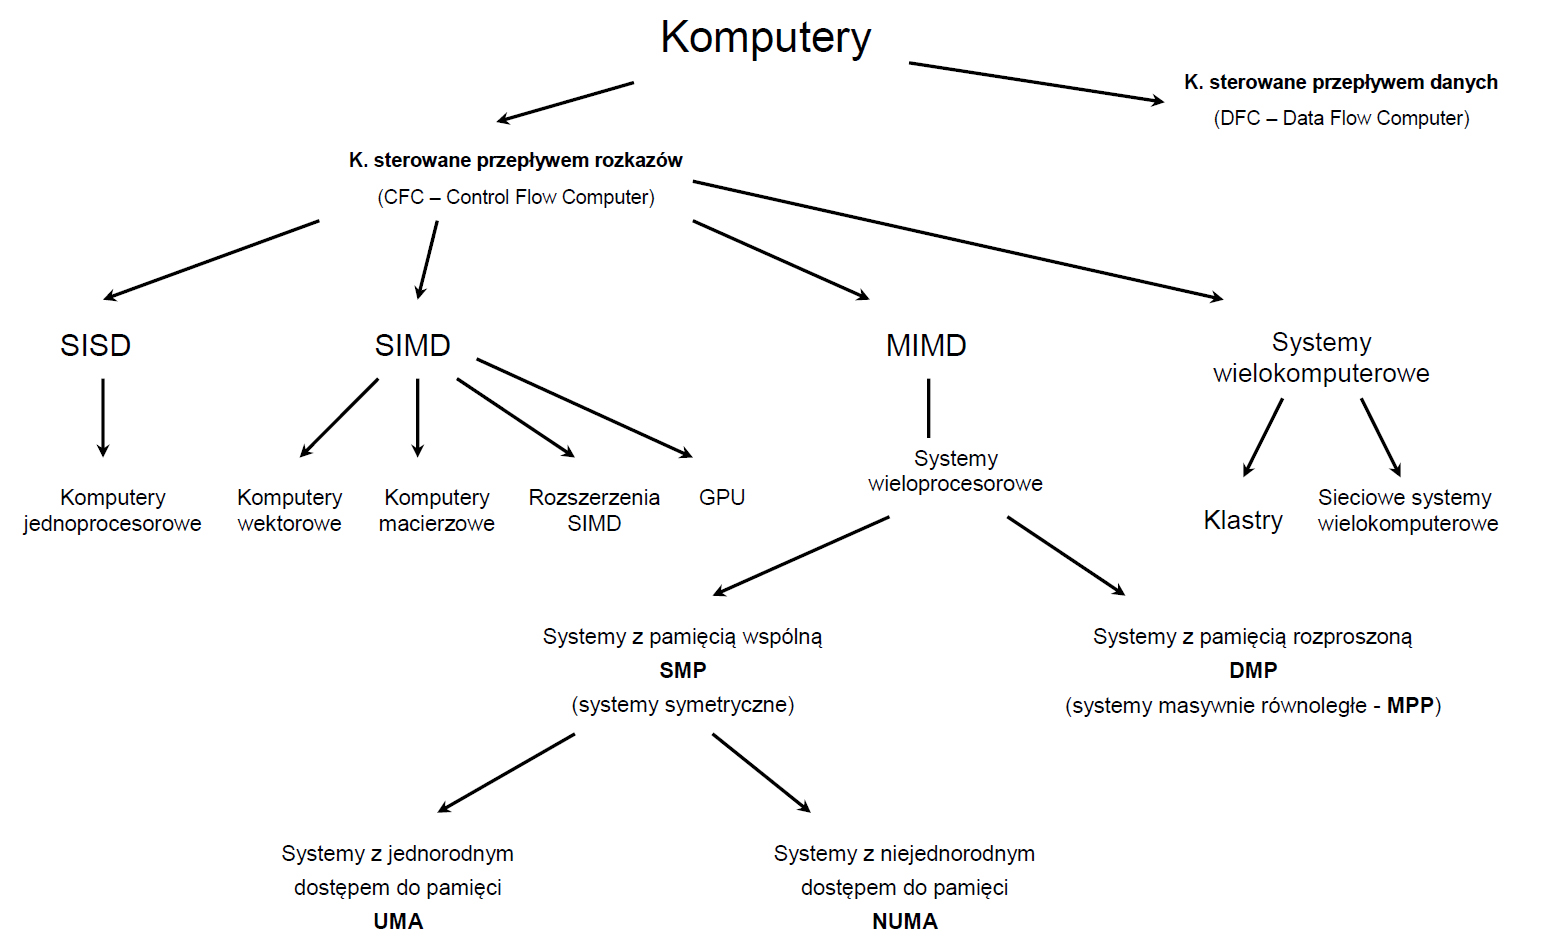
\includegraphics[width=16cm]{klasyfikacja}
\pagebreak
	
\section{Architektura SIMD}
	\subsection{Co to jest?}
		Cecha wyróżniająca dla programisty - rozkazy wektorowe (rozkazy z argumentami wektorowymi).\\
		Dwa różne podejścia do sprzętowej realizacji rozkazów wektorowych:
		\begin{itemize}
			\item Komputery (procesory) macierzowe
			\item Komputery wektorowe
		\end{itemize}
		Idee realizacji obu (macierzowy i wektorowy):\\
		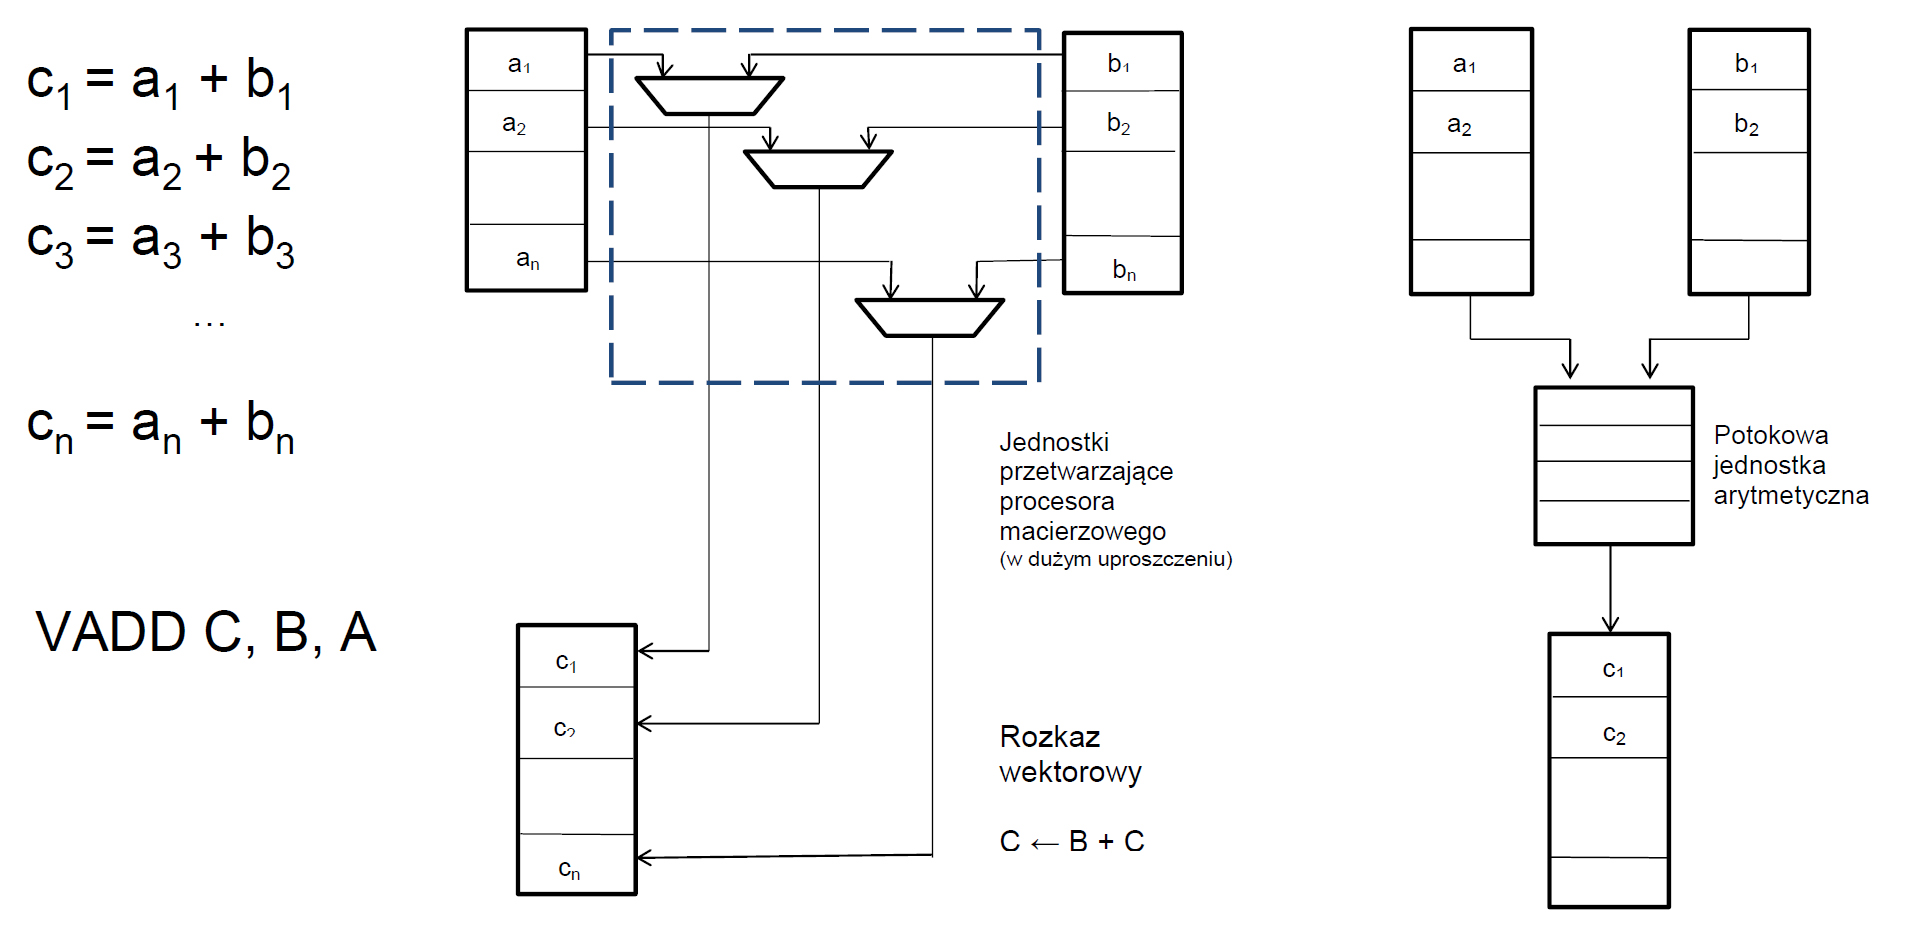
\includegraphics[width=16cm]{wektor_macierz}\\
	\subsection{Komputery wektorowe}
		\subsubsection{Lokalizacja wektorów danych}
			\begin{itemize}
				\item Pamięć operacyjna
				\item Rejestry wektorowe
			\end{itemize}
		\subsubsection{Przykład rozkazu}
			Rozkaz dodawania wektorów: VADDF A,B,C,n\\
			Czas wykonania: $t_{w}=t_{start}+(n-1)\times\tau$\\
			W komputerze macierzowym czas wykonywania tego rozkazu jest równy \emph{const}.
		
		\subsubsection{Przyspieszenie}
			Przyspieszenie jest stosunkiem czasu wykonywania w komputerze klasycznym (szeregowo) do czasu wykonywania w komputerze wektorowym.\\\\
			$a=lim_{n \to \infty}\frac{15\times\tau\times n}{t_{start}+(n-1)\times\tau}=15$
		
		\subsubsection{Przepustowość}
			Przepustowość (moc obliczeniowa) jest stosunkiem ilości operacji zmiennoprzecinkowych do czasu ich wykonania.\\\\
			$Przep=lim_{n \to \infty}\frac{n}{t_{start}+(n-1)\times\tau}=\frac{1}{\tau}$
	
		\subsubsection{Podsumowanie}
			\begin{enumerate}
				\item Hardware
				\begin{itemize}
					\item rozkazy wektorowe
					\item duża liczba potokowych jednostek arytmetycznych
					\item duża liczba rejestrów
				\end{itemize}
				\item Software
				\begin{itemize}
					\item klasyczne języki: Fortran, C
					\item klasyczne algorytmy
					\item kompilatory wektoryzujące
				\end{itemize}
			\end{enumerate}

		\subsubsection{Zastosowanie}
			\begin{itemize}
				\item Numeryczna symulacja ośrodków ciągłych
				\item Równania różniczkowe, równania różnicowe, układy równań algebraicznych (rachunek macierzowy)
				\item Dziedziny zastosowań:
				\begin{itemize}
					\item prognozowanie pogody
					\item symulacja aerodynamiczna
					\item sejsmiczne poszukiwania ropy naftowej i innych surowców
					\item symulacja reakcji jądrowych
					\item medycyna i farmacja
					\item obliczenia inżynierskie dużej skali
				\end{itemize}
			\end{itemize}
		
	\subsection{Komputery macierzowe}
		\subsubsection{Co to jest?}
			Architektura komputerów macierzowych - model SIMD w dwóch wariantach:
			\begin{itemize}
				\item SIMD - DM (z pamięcią rozproszoną)
				\item SIMD - SM (z pamięcią wspólną)
			\end{itemize}
		
		\subsubsection{Elementy komputera macierzowego}
			\begin{enumerate}
				\item \textbf{Jednostka sterująca} - procesor wykonujący rozkazy sterujące i skalarne oraz inicjujący wykonanie rozkazów wektorowych w sieci elementów przetwarzających.
				\item \textbf{Elementy przetwarzające} (procesorowe) - jednostki arytmetyczno-logiczne wykonujące operacje elementarne rozkazów wektorowych.
				\item \textbf{Sieć łącząca} - łączy elementy przetwarzające między sobą lub z modułami pamięci operacyjnej; warianty:
				\begin{itemize}
					\item sieć statyczna: pierścień, gwiazda, krata, drzewo, hipersześcian
					\item sieć dynamiczna: jednostopniowa, wielostopniowa
				\end{itemize}
			\end{enumerate}
		
		\subsubsection{Podsumowanie}
			\begin{itemize}
				\item Architektura SIMD
				\item Jednostka sterująca + jednostka macierzowa
				\item Rozkazy wektorowe - wykonywane synchronicznie w sieci (macierzy) EP
				\item Skomplikowana wymiana danych między EP
				\item Trudne programowanie - konieczność tworzenia nowych wersji algorytmów
			\end{itemize}
		
	\subsection{Model SIMD w procesorach superskalarnych}
		\subsubsection{Technologia MMX}
			\begin{itemize}
				\item 8 rejestrów 64-bitowych MMX
				\item Nowe typy danych
				\item Rozszerzony zestaw instrukcji (57 instrukcji)
				\item Realizacja operacji na krótkich wektorach wg modelu SIMD
			\end{itemize}
	\subsection{Technologia SSE}
		\begin{itemize}
			\item 8 rejestrów 128-bitowych
			\item Osiem 16-bitowych argumentów (elementów wektora) typu integer
			\item Cztery 32-bitowe argumenty integer/fplub dwa 64-bitowe
			\item Operacje zmp na 4-elementowych wektorach liczb 32-bit (pojed. prec.)
		\end{itemize}
		
\section{Karty graficzne i architektura CUDA}
	\subsection{Charakterystyka}
		\begin{itemize}
			\item GPU - Graphics Processing Unit
			\item Wcześniejsze GPU - specjalizowane języki (HLSL, GLSL czy NVIDIA Cg), tylko rendering
			\item CUDA (Compute Unified Device Architecture) -architektura wielordzeniowych procesorów graficznych (GPU)
			\item Uniwersalna architektura obliczeniowa połączona z równoległym modelem programistycznym
			\item wsparcie dla języków C/C++
			\item GPGPU = GPU + CUDA
			\item CUDA - obsługiwana przez karty graficzne GeForce i GeForce Mobile od serii 8 (GeForce 8800), nowsze układy z rodzin Tesla i Quadro, Fermi, obecnie Kepler
		\end{itemize}
	\subsection{Architektura CUDA}
		\begin{itemize}
			\item W miejsce oddzielnych potoków przetwarzających wierzchołki i piksele wprowadzenie uniwersalnego procesora przetwarzającego wierzchołki, piksele i ogólnie geometrię, a także uniwersalne programy obliczeniowe
			\item Wprowadzenie procesora wątków eliminującego „ręczne” zarządzanie rejestrami wektorowymi
			\item Wprowadzenie modelu SIMT (single-instruction multiple-thread), w którym wiele niezależnych wątków wykonuje równocześnie tę samą instrukcję
			\item Wprowadzenie współdzielonej pamięci oraz mechanizmów synchronizacji wątków (barrier synchronization) dla komunikacji między wątkami
		\end{itemize}
	\subsection{Multiprocesor strumieniowy}
		\begin{itemize}
			\item 8 rdzeni C1 -C8 (SP)
			\item podręczna pamięć instrukcji (ang. instruction cache),
			\item podręczna pamięć danych (ang. constant cache) -pamięć tylko do odczytu,
			\item pamięć współdzielona (ang. shared memory)
			\item 16 384 rejestry,
			\item jednostka arytmetyczna wykonująca obliczenia zmiennoprzecinkowe podwójnej precyzji (fp64),
			\item dwie jednostki arytmetyczne przeznaczone do obliczania funkcji specjalnych (ang. special function unit),
			\item pamięć globalna
		\end{itemize}
	\subsection{Model programistyczny CUDA}
		\begin{itemize}
			\item Specjalny kompilator NVCC
			\item Podział programu na kod wykonywany przez procesor (ang. Host code) i przez urządzenie (kartę graficzną) (ang. Device code) - kernel
			\item Realizacja operacji równoległych według modelu SIMT (Single Instruction Multiple Threading)
		\end{itemize}
	\subsection{Wykonanie obliczeń z użyciem architektury CUDA (5 faz)}
		\begin{enumerate}
			\item Przydzielenie w pamięci globalnej obszaru pamięci dla danych, na których będą wykonywane obliczenia przez kernel.
			\item Przekopiowanie danych do przydzielonego obszaru pamięci.
			\item Zainicjowanie przez CPU obliczeń wykonywanych przez GPU, tj. wywołanie kernela.
			\item Wykonanie przez wątki (z użyciem GPU) obliczeń zdefiniowanych w kernelu.
			\item Przekopiowanie danych z pamięci globalnej do pamięci operacyjnej.
		\end{enumerate}
	\subsection{CUDA procesor (rdzeń)}
		\begin{itemize}
			\item Potokowa jednostka arytmetyczna zmp
			\item Potokowa jednostka arytmetyczna stp
			\item Ulepszona realizacja operacji zmp FMA (fused multiply-add) dla pojedynczej i podwójnej precyzji
		\end{itemize}

	\pagebreak
	\section{Wątki}
		\begin{itemize}
			\item Wątek reprezentuje pojedynczą operację (a single work unit or operation)
			\item Wątki są automatycznie grupowane w bloki, maksymalny rozmiar bloku = 512 wątków (w architekturze Fermi i wyższych –1024 wątki).
			\item Bloki grupowane są w siatkę (grid -kratę)
			\item Grupowanie wątków –bloki o geometrii 1, 2 lub 3-wymiarowej
			\item Grupowanie bloków –siatka (grid) o geometrii 1, 2-wymiarowej
			\item Wymaga się, aby bloki wątków tworzących siatkę mogły się wykonywać niezależnie: musi być możliwe ich wykonanie w dowolnym porządku, równolegle lub szeregowo.
		\end{itemize}
		\subsection{Grupowanie wątków w bloki i siatkę}
			\begin{itemize}
				\item Siatka o geometrii jednowymiarowej (trzy bloki wątków)
				\item Każdy blok -geometria dwuwymiarowa (wymiary 2 x 3)
			\end{itemize}
		\subsection{Sprzętowa organizacja wykonywania wątków}
			\begin{itemize}
				\item Przy uruchomieniu kernel’awszystkie bloki tworzące jego siatkę obliczeń są rozdzielane pomiędzy multiprocesory danego GPU
				\item Wszystkie wątki danego bloku są przetwarzane w tym samym multiprocesorze
				\item W danej chwili (cyklu) pojedynczy rdzeń multiprocesora wykonuje jeden wątek programu
				\item Multiprocesor tworzy, zarządza, szereguje i wykonuje wątki w grupach po 32, nazywanych wiązkami (warp).
				\item Wiązki są szeregowane do wykonania przez warp scheduler. Wiązka wątków jest wykonywana jako jeden wspólny rozkaz (analogia do rozkazu SIMD, tzn. rozkazu wektorowego)
				\item Sposób wykonania wiązki wątków (rozkazu SIMD) zależy od budowy multiprocesora:
				\begin{itemize}
					\item Dla architektury Fermi (32 procesory w jednym multiprocesorze / 2 warp-scheduler’y= 16 procesorów na 1 wiązkę) wiązka jest wykonywana jako 2 rozkazy -wiązka jest dzielona na dwie połówki (half –warp) wykonywane jako 2 rozkazy (te same, ale na dwóch zestawach danych).
					\item Dla architektury Tesla (8 procesorów w jednym multiprocesorze, 1 warp-scheduler) wiązka jest dzielona na cztery ćwiartki (quarter-warp) wykonywane jako 4 kolejne rozkazy (te same, ale na czterech zestawach danych).
				\end{itemize}
				\item Konstrukcja warp scheduler’a umożliwia uruchomienie wielu wiązek wątków współbieżnie - warp scheduler pamięta wtedy adresy wiązek, przypisane im rozkazy SIMD oraz ich stan (gotowość do wykonania lub stan oczekiwania na pobranie danych z pamięci).
				\item Współbieżne uruchomienie wielu wiązek pozwala zmniejszyć straty związane z oczekiwaniem na dane (zwykle długi czas dostępu do pamięci).
			\end{itemize}
			
\section{Rodzaje pamięci multiprocesora}
	\begin{itemize}
		\item \textbf{pamięć globalna} – duża pamięć, o czasie życia aplikacji (dane umieszczone w tej pamięci są usuwane po zakończeniu aplikacji), dostępna dla każdego wątku w dowolnym bloku, ale o dość długim czasie dostępu wynoszącym ok. 400-600 taktów zegara,
		\item \textbf{pamięć współdzielona} – niewielka pamięć o czasie życia bloku (zakończenie działania bloku powoduje usunięcie danych w niej przechowywanych), dostępna dla każdego wątku w bloku dla którego jest dedykowana, o bardzo krótkim czasie dostępu,
		\item \textbf{pamięć stałych} – niewielki fragment pamięci globalnej, który jest cache-owany, przez co dostęp do niego jest bardzo szybki. Jest ona tylko do odczytu. Czas życia pamięci stałych oraz jej dostępność jest taka sama jak pamięci globalnej,
		\item \textbf{rejestry} – niewielka, bardzo szybka pamięć o czasie życia wątku (po zakończeniu wątku dane z rejestrów są usuwane). Tylko jeden wątek może w danym momencie korzystać z danego rejestru,
		\item \textbf{pamięć lokalna i pamięć tekstur} – podobnie jak w przypadku pamięci stałych, są to dedykowane fragmenty pamięci globalnej. Pamięć lokalna jest wykorzystywana do przechowywania danych lokalnych wątku, które nie mieszczą się w rejestrach, a pamięć tekstur posiada specyficzne metody adresowania i cache-owanie specyficzne dla zastosowań graficznych.
	\end{itemize}
	
\section{Systemy wieloprocesorowe}
	\subsection{Rodzaje}
		\begin{itemize}
			\item systemy z pamięcią wspólną
			\item systemy z pamięcią rozproszoną
		\end{itemize}
		\subsubsection{Z pamięcią wspólną}
			\begin{itemize}
				\item Systemy z jednorodnym dostępem do pamięci (UMA – Uniform Memory Access)
				\item Systemy z niejednorodnym dostępem do pamięci (NUMA – Non 	- Uniform Memory Access)
				\item Klasyfikacja:
				\begin{itemize}
					\item Systemy ze wspólną magistralą
					\item Systemy wielomagistralowe
					\item Systemy z przełącznicą krzyżową
					\item Systemy z wielostopniową siecią połączeń
					\item Systemy z pamięcią wieloportową
					\item Systemy z sieciami typu punkt - punkt
				\end{itemize}
			\end{itemize}
		\subsubsection{Systemy ze wspólną magistralą}
			\begin{itemize}
				\item prostota konstrukcji – niska złożoność układowa całości
				\item niski koszt
				\item łatwość rozbudowy – dołączenia kolejnego procesora, ale tylko w ograniczonym zakresie
				\item ograniczona złożoność magistrali (jej szybkość jest barierą)
				\item niska skalowalność
			\end{itemize}
	\subsection{Skalowalność}
		\textbf{System skalowalny} - System, w którym dodanie pewnej liczby procesorów prowadzi do proporcjonalnego przyrostu mocy obliczeniowej.
	\subsection{Protokół MESI}
		\begin{itemize}
			\item I - invalid
			\item S - shared
			\item E - exclusive
			\item M - modified
		\end{itemize}
	\subsection{Systemy wielomagistralowe}
		\begin{itemize}
			\item Wielokrotnie zwiększona przepustowość
			\item Konieczność stosowania układu arbitra do sterowania dostępem do magistral
			\item Rozwiązania kosztowne
			\item Zadania każdego przełącznika
			\begin{itemize}
				\item Rozwiązywanie konfliktów dostępu do tego samego modułu pamięci
				\item Zapewnienie obsługi równoległych transmisji, krzyżujących się w przełączniku
			\end{itemize}
		\end{itemize}
	\subsection{Systemy UMA}
		\begin{itemize}
			\item Symetryczna architektura – jednakowy dostęp procesorów do pamięci operacyjnej oraz we/wy
			\item Utrzymanie spójności pamięci podręcznych (cache):
			\begin{itemize}
				\item snooping - metoda starsza i mało skalowalna (głównie w systemach ze wspólną magistralą)
				\item katalog - metoda lepiej skalowalna, stosowana razem z sieciami typu punkt - punkt
			\end{itemize}
			\item Łatwe programowanie (realizacja algorytmów równoległych)
			\item Niska skalowalność
		\end{itemize}
	\subsection{Systemy NUMA}
		\begin{itemize}
			\item PaO fizycznie rozproszona, ale logicznie wspólna
			\item Niejednorodny dostęp do pamięci - PaO lokalna, PaO zdalna
			\item Utrzymanie spójności pamięci podręcznych (cache) - katalog
			\item Hierarchiczna organizacja: procesor – węzeł (system UMA) – system NUMA
			\item Zalety modelu wspólnej pamięci dla programowania
			\item Dobra efektywność dla aplikacji o dominujących odczytach z nielokalnej pamięci
			\item Gorsza efektywność dla aplikacji o dominujących zapisach do nielokalnej pamięci
			\item Skalowalność: 1024 – 2560 rdzeni
		\end{itemize}
	\subsection{Systemy SMP}
		\begin{itemize}
			\item Symetryczna architektura – jednakowy dostęp procesorów do pamięci operacyjnej oraz we/wy (na poziomie fizycznych przesyłów –
			tylko w systemach wieloprocesorowe z pamięcią wspólną fizycznie - UMA)
			\item Utrzymanie spójności pamięci podręcznych (cache):
			\begin{itemize}
				\item systemy UMA - snooping lub katalog
				\item systemy NUMA - katalog
			\end{itemize}
			\item Łatwe programowanie (realizacja algorytmów równoległych)
			\item Niska (UMA) i średnia (NUMA) skalowalność
		\end{itemize}